\chapter{SYSTEM DESIGN}

\section{System Architecture}

The VoteDesk system follows the Model-View-Controller (MVC) architectural pattern provided by the Laravel framework. This architecture ensures a clear separation of concerns between data management, business logic, and the presentation layer.

\begin{figure}[H]
\centering
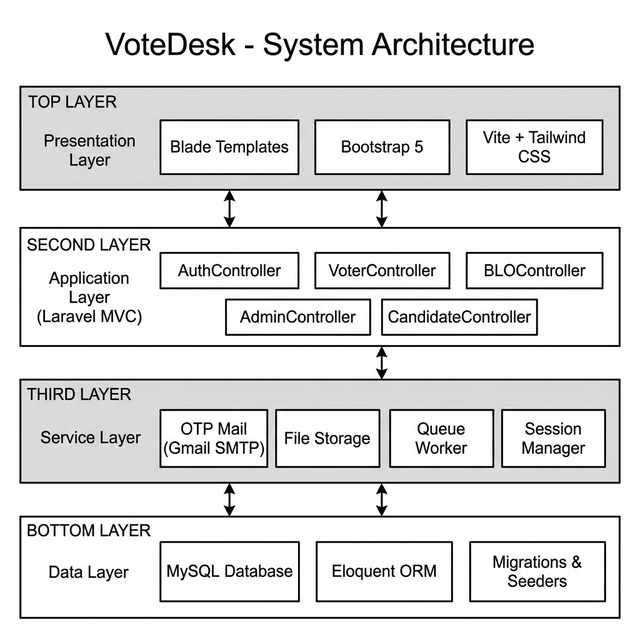
\includegraphics[width=\textwidth,height=0.75\textheight,keepaspectratio]{system_architecture.png}
\caption{VoteDesk System Architecture Diagram}
\label{fig:architecture}
\end{figure}

The architecture diagram illustrates how the frontend, backend, and external service components interact.

The system is structured into four primary layers:

\begin{enumerate}
    \item \textbf{Presentation Layer:} Blade-templated HTML views served by Laravel, styled with Bootstrap 5 and Tailwind CSS 4, with JavaScript assets compiled by Vite.
    \item \textbf{Application Layer:} Laravel controllers handle HTTP requests, enforce business rules, and return appropriate responses. Middleware enforces role-based access control.
    \item \textbf{Service Layer:} Supporting services include the Laravel Mail system (Gmail SMTP), Laravel Storage (for voter photo capture), and the Queue worker for asynchronous email dispatch.
    \item \textbf{Data Layer:} MySQL database accessed through Eloquent ORM. Migrations maintain a version-controlled schema, and Seeders initialise default data.
\end{enumerate}

\section{Use Case Diagram}

\begin{figure}[H]
\centering
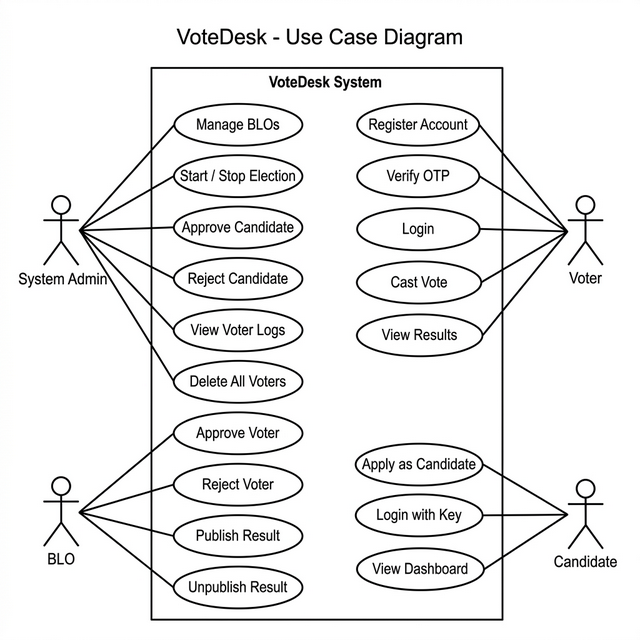
\includegraphics[width=\textwidth,height=0.75\textheight,keepaspectratio]{use_case.png}
\caption{VoteDesk Use Case Diagram}
\label{fig:usecase}
\end{figure}

The diagram shows how different users interact with the digital election system.

\section{Database Design}

\begin{figure}[H]
\centering
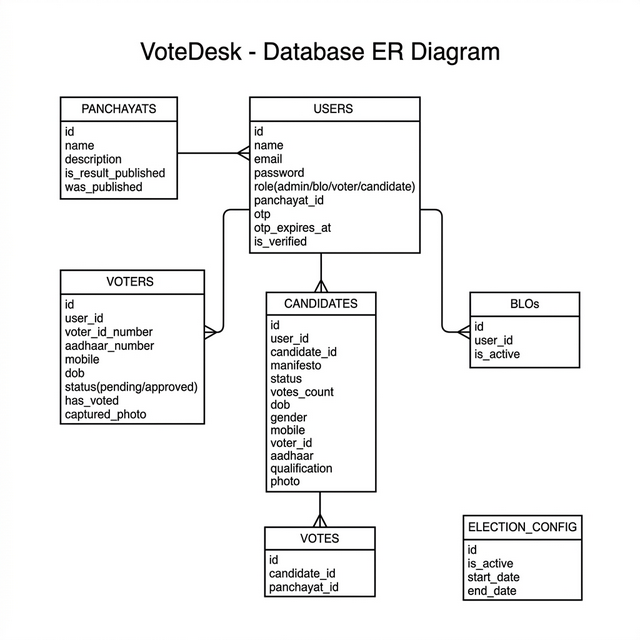
\includegraphics[width=\textwidth,height=0.75\textheight,keepaspectratio]{er_diagram.png}
\caption{VoteDesk Entity Relationship (ER) Diagram}
\label{fig:er}
\end{figure}

The entity relationship diagram represents the database schema, including tables, primary keys, and relations among user roles.

\section{Class Diagram}

\begin{figure}[H]
\centering
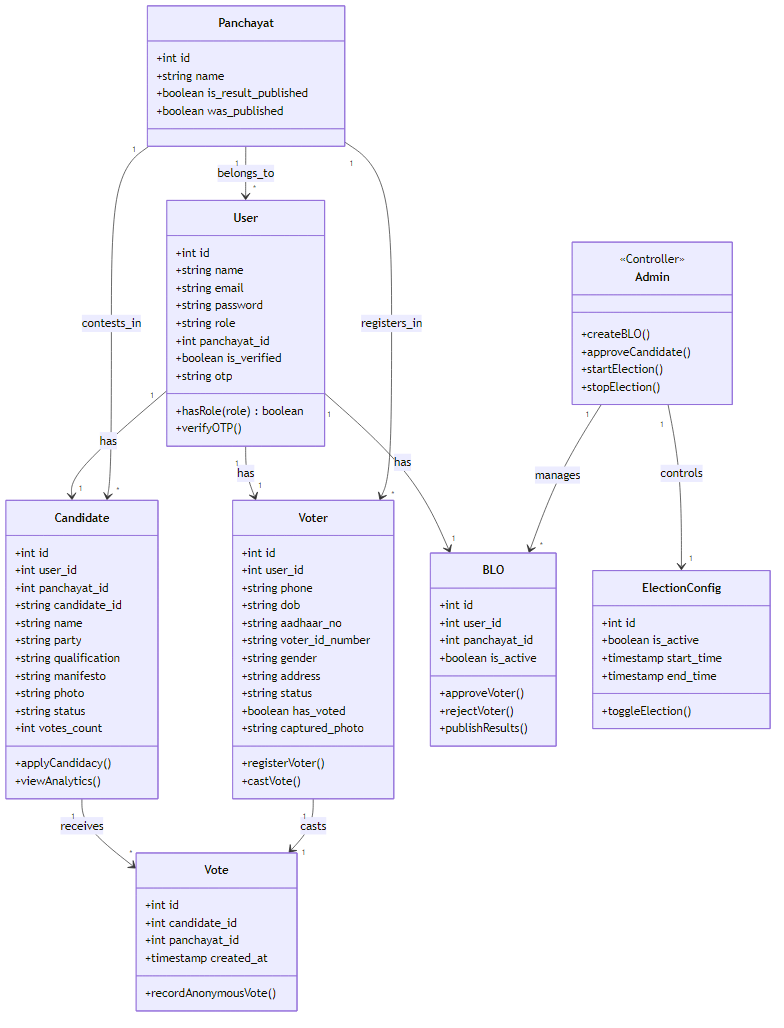
\includegraphics[width=\textwidth,height=0.75\textheight,keepaspectratio]{diagrams/class_diagram.png}
\caption{VoteDesk System Class Diagram}
\label{fig:class}
\end{figure}

The class diagram illustrates the structural design of the VoteDesk system, showing the main classes, their attributes, methods, and relationships.

\section{Sequence Diagrams}

\subsection{Voter Registration and OTP Verification}

\begin{figure}[H]
\centering
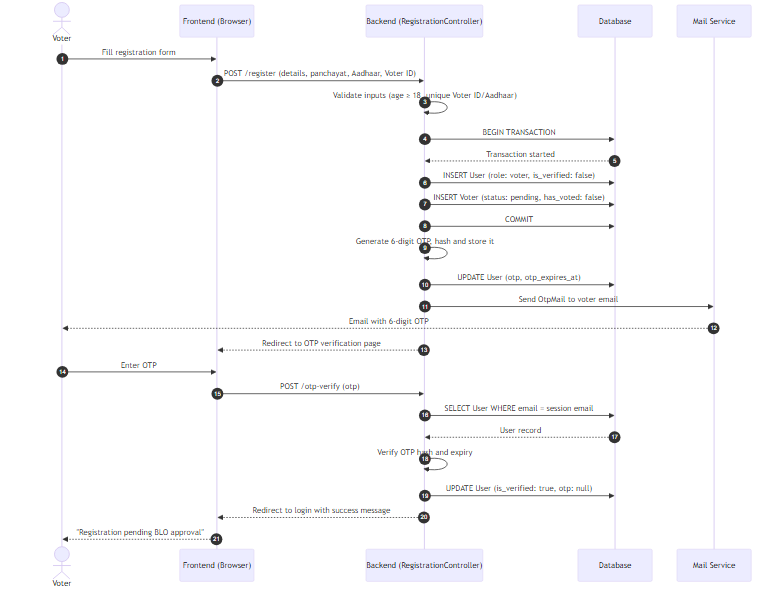
\includegraphics[width=\textwidth,height=0.75\textheight,keepaspectratio]{diagrams/sequence_diagram_1.png}
\caption{Sequence Diagram: Voter Registration and OTP Email Verification}
\label{fig:seq_registration}
\end{figure}

This diagram shows the sequence of interactions during the voter registration and OTP verification process.

\subsection{Vote Casting Process}

\begin{figure}[H]
\centering
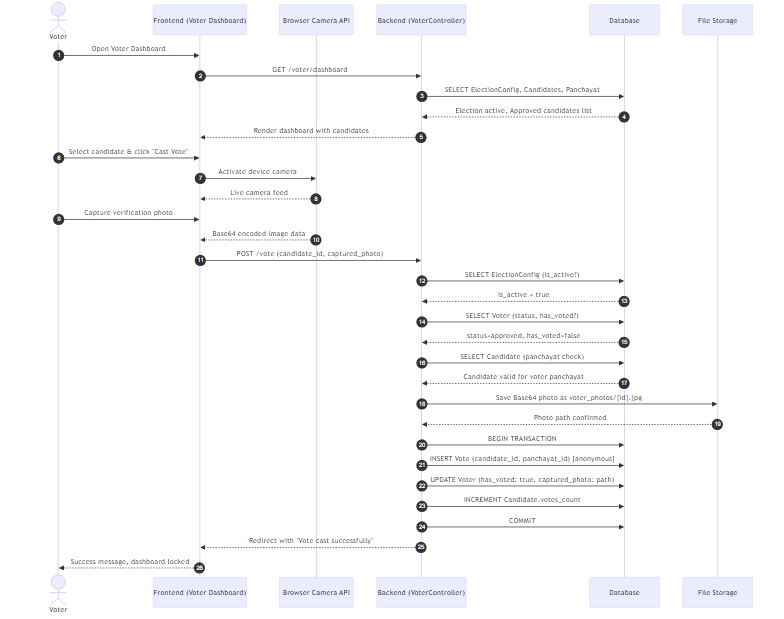
\includegraphics[width=\textwidth,height=0.75\textheight,keepaspectratio]{diagrams/sequence_diagram_2.png}
\caption{Sequence Diagram: Vote Casting with Real-Time Photo Capture}
\label{fig:seq_vote}
\end{figure}

This diagram illustrates the sequence of messages and database transactions during the secure vote casting process.

\subsection{Candidate Approval and Result Publication}

\begin{figure}[H]
\centering
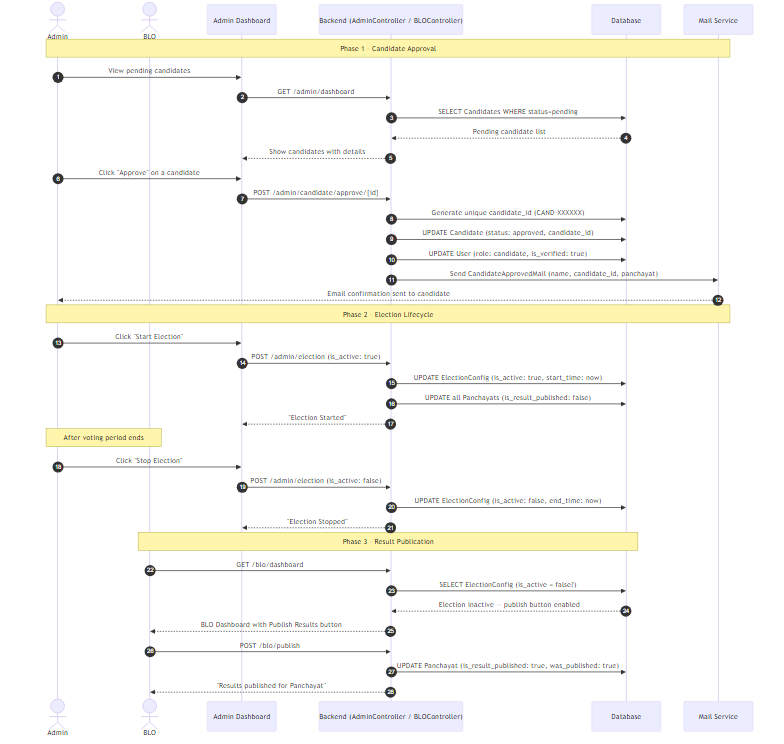
\includegraphics[width=\textwidth,height=0.75\textheight,keepaspectratio]{diagrams/sequence_diagram_3.png}
\caption{Sequence Diagram: Candidate Approval and Election Results Publication}
\label{fig:seq_results}
\end{figure}

This diagram displays the multi-role interactions for candidate approval, election management, and result publication.

\section{Module Design}

The system is divided into six primary functional modules:

\begin{itemize}
    \item \textbf{Authentication Module:} Handles multi-role login with tab-based portal selection, OTP email verification, forgot password with OTP reset, and session-based role management.
    \item \textbf{Voter Registration Module:} Collects voter identity details, validates Aadhaar and Voter ID uniqueness, sends OTP, and creates a pending voter record awaiting BLO approval.
    \item \textbf{BLO Management Module:} Enables the admin to create BLO accounts assigned to a specific panchayat. BLOs approve or reject pending voter applications within their panchayat boundary.
    \item \textbf{Candidate Management Module:} Processes public candidate applications with photo upload, enforces admin approval workflow, generates a unique Candidate Key, and sends approval email.
    \item \textbf{Voting Module:} Presents approved candidates to the voter, captures a real-time photograph via the device camera, wraps the vote creation and voter update in a database transaction, and increments the candidate vote count atomically.
    \item \textbf{Results Module:} BLOs publish results for their panchayat after the election ends. The public results page displays candidate rankings with vote counts, grouped by panchayat.
\end{itemize}

\subsection{Module Interaction Diagram}

\begin{figure}[H]
\centering
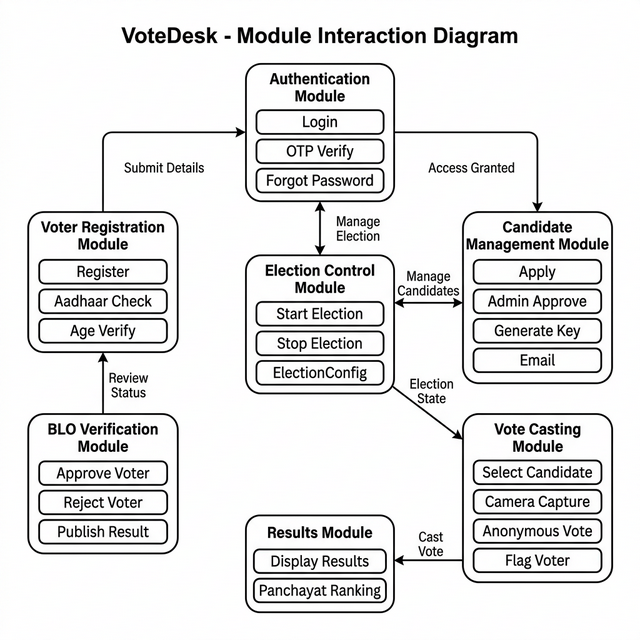
\includegraphics[width=\textwidth,height=0.75\textheight,keepaspectratio]{module_interaction.png}
\caption{VoteDesk Module Interaction Diagram}
\label{fig:module_int}
\end{figure}

This module interaction diagram illustrates how data flows between the six primary functional modules of the system.

\subsection{Voter Registration and Approval Flow}

\begin{enumerate}
    \item Voter navigates to the Registration page and submits personal details.
    \item System validates data and creates a User record (role: voter) and a Voter record (status: pending).
    \item A 6-digit OTP is generated, hashed, and dispatched to the voter's email via Gmail SMTP.
    \item Voter enters the OTP on the verification page. System verifies hash and marks user as \texttt{is\_verified = true}.
    \item BLO logs into their dashboard and views the pending voter in their panchayat's list.
    \item BLO approves the voter. Voter status is updated to \texttt{approved}.
    \item Voter can now log in and cast their vote.
\end{enumerate}

\subsection{Vote Casting Flow}

\begin{enumerate}
    \item Approved voter logs into the Voter Dashboard.
    \item System verifies election is active (\texttt{ElectionConfig.is\_active = true}).
    \item Voter views candidates from their registered panchayat.
    \item Voter selects a candidate and activates the camera to capture a verification photo.
    \item On form submission, the system validates: election active, voter approved, voter has not voted, candidate belongs to voter's panchayat.
    \item Within a database transaction: an anonymous Vote record is created, the voter's \texttt{has\_voted} flag is set to true, the captured photo is stored, and the candidate's \texttt{votes\_count} is incremented.
    \item Voter is redirected to their dashboard with a success notification.
\end{enumerate}

\section{System Pipeline / Workflow Diagram}

\begin{figure}[H]
\centering
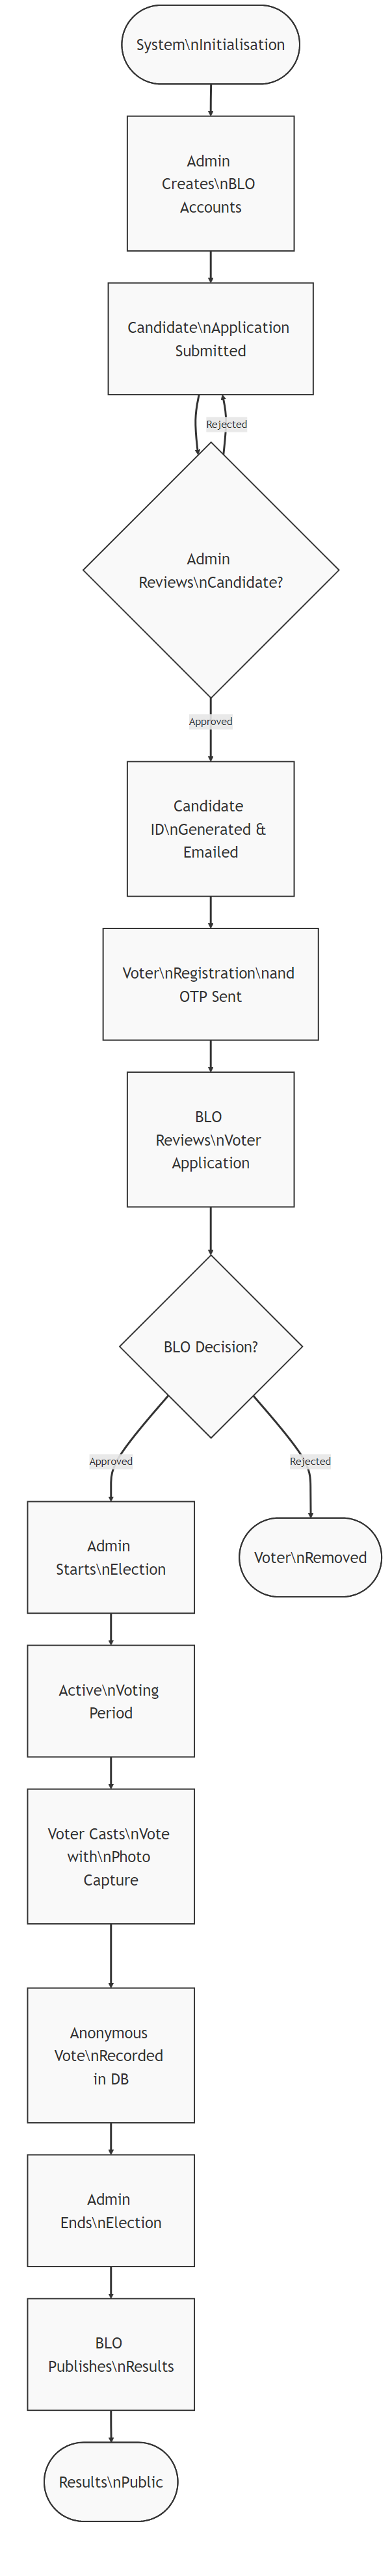
\includegraphics[width=\textwidth,height=0.75\textheight,keepaspectratio]{diagrams/system_pipeline.png}
\caption{VoteDesk System Pipeline / Election Lifecycle Workflow}
\label{fig:pipeline}
\end{figure}

The system pipeline workflow diagram outlines the complete election lifecycle from initialisation to public result announcement.

\section{Activity Diagram}

\begin{figure}[H]
\centering
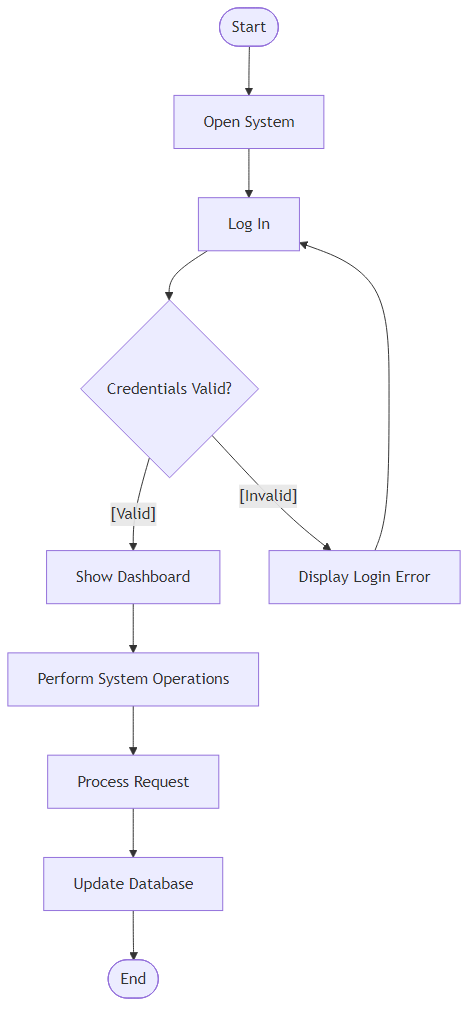
\includegraphics[width=\textwidth,height=0.75\textheight,keepaspectratio]{diagrams/activity_diagram.png}
\caption{Activity Diagram of System Workflow}
\label{fig:activity}
\end{figure}

The activity diagram describes the sequential workflow followed by a user during the digital election process.

\section{System Screenshots}

The following screenshots represent the key interfaces of the VoteDesk system.

\begin{figure}[H]
\centering

\includegraphics[width=\textwidth,height=0.75\textheight,keepaspectratio]{screenshots/login_ss.png}
\caption{Screenshot 1: Login Interface}
\label{fig:login_ss}
\end{figure}

\begin{figure}[H]
\centering
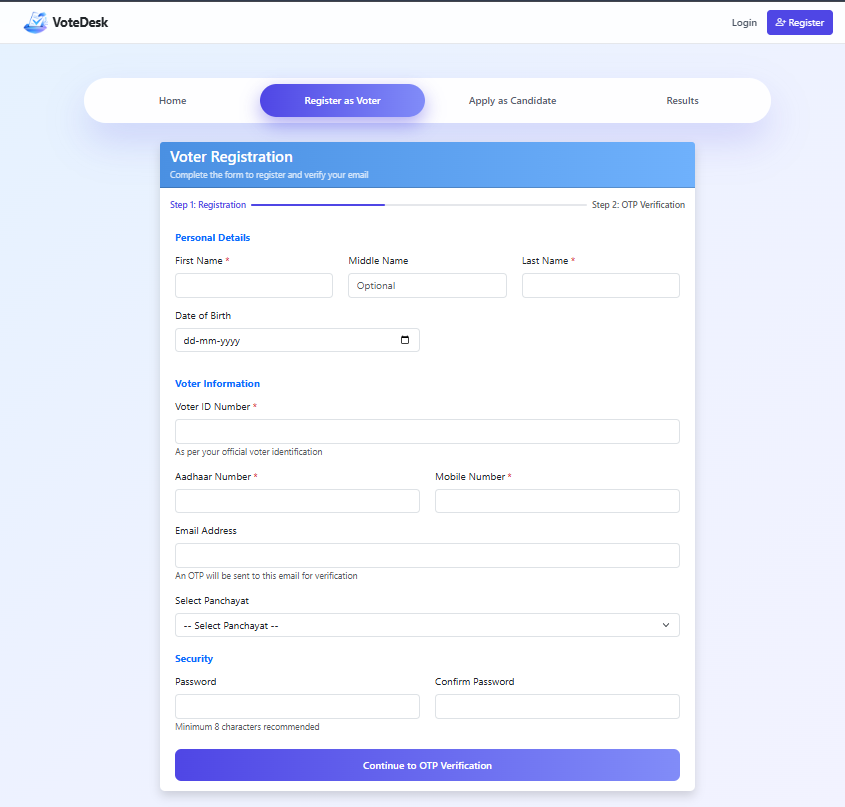
\includegraphics[width=\textwidth,height=0.75\textheight,keepaspectratio]{screenshots/voter_register_ss.png}
\caption{Screenshot 2: Voter Registration Form}
\label{fig:voter_register}
\end{figure}

\begin{figure}[H]
\centering
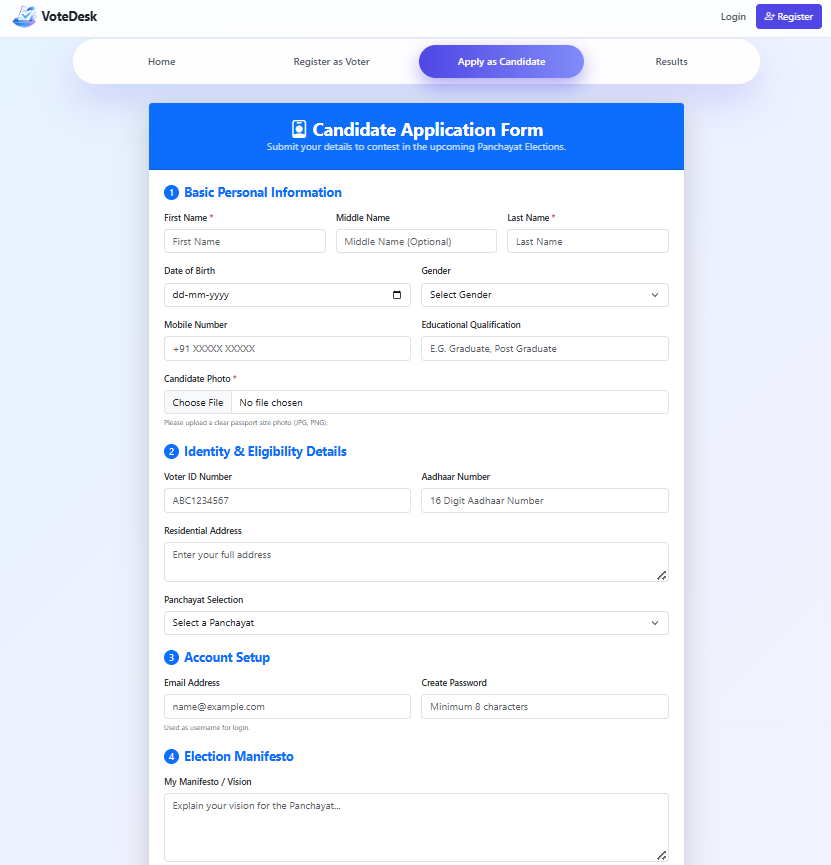
\includegraphics[width=\textwidth,height=0.75\textheight,keepaspectratio]{screenshots/candiate_register_ss.png}
\caption{Screenshot 3: Candidate Registration Form}
\label{fig:candidate_register}
\end{figure}

\begin{figure}[H]
\centering

\includegraphics[width=\textwidth,height=0.75\textheight,keepaspectratio]{screenshots/admin_dash_ss.png}
\caption{Screenshot 4: Admin Dashboard Overview}
\label{fig:admin_dash_ss}
\end{figure}

\begin{figure}[H]
\centering
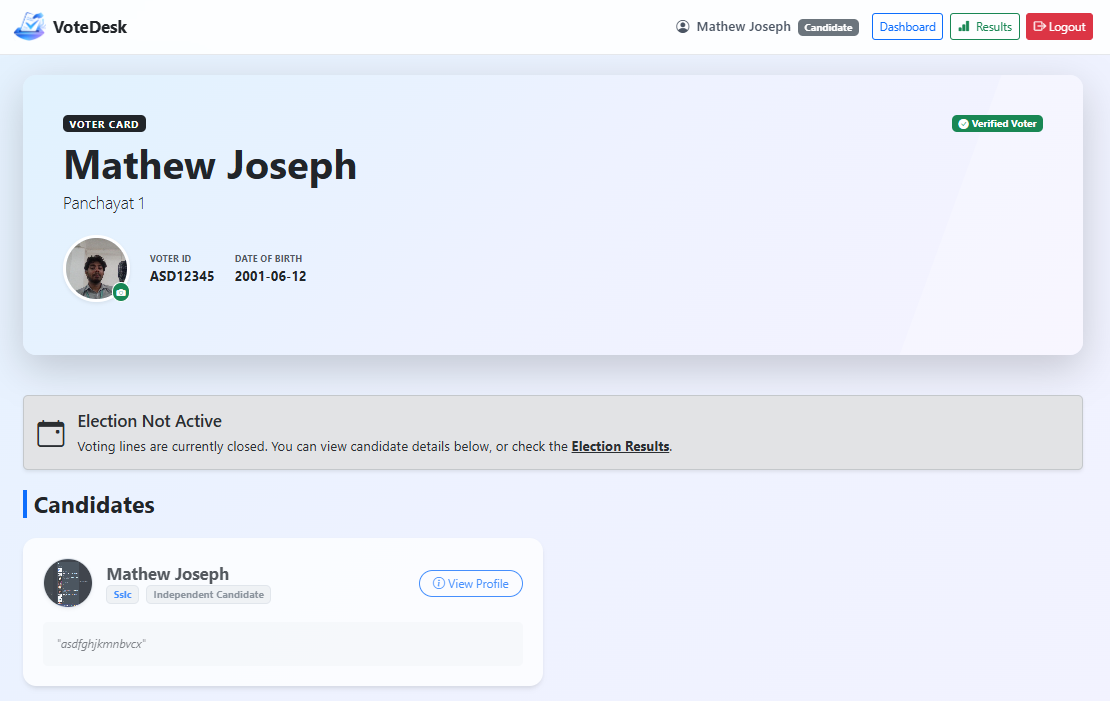
\includegraphics[width=\textwidth,height=0.75\textheight,keepaspectratio]{screenshots/voter_dash_ss.png}
\caption{Screenshot 5: Voter Casting Interface}
\label{fig:voter_dash_ss}
\end{figure}
